\section{Opgave 5 - Count '1' using the for loop}
\begin{enumerate}
	\item[1)]
	Vi skriver koden for en process, som kan tælle antallet af 1'er i et 8bit input, og vise det på et 7-segment output. Koden er vist på figur \ref{lst:count} og på figur \ref{fig:1count0}, \ref{fig:1count6} og \ref{fig:1count8}  ses resultatet på DE2-boardet hvor HEX0 er output og SW[7-0] er input.\\
	\begin{lstlisting}[caption={Behavioral style kode for en '1'-counter},label={lst:count}]
	library ieee;
	use ieee.std_logic_1164.all;
	use ieee.numeric_std.all;
	
	entity countOne is
	port(input : in std_logic_vector(7 downto 0);
	segA : out std_logic_vector(6 downto 0));
	end countOne;
	
	architecture selection of countOne is
	begin
	
	count: process (input)
	variable A : std_logic_vector(3 downto 0);
	begin
	A := "0000";
	for i in 7 downto 0 loop
	if input(i) = '1' then A := std_logic_vector(unsigned(A) + 1);
	end if;
	end loop;
	
	case A is
	when "0000" => segA <= "0000001"; -- 0
	when "0001" => segA <= "1001111"; -- 1
	when "0010" => segA <= "0010010"; -- 2
	when "0011" => segA <= "0000110"; -- 3
	when "0100" => segA <= "1001100"; -- 4
	when "0101" => segA <= "0100100"; -- 5
	when "0110" => segA <= "0100000"; -- 6
	when "0111" => segA <= "0001111"; -- 7
	when "1000" => segA <= "0000000"; -- 8
	when "1001" => segA <= "0001100"; -- 9
	when "1010" => segA <= "0001000"; -- A
	when "1011" => segA <= "1100000"; -- B
	when "1100" => segA <= "0110001"; -- C
	when "1101" => segA <= "1000010"; -- D
	when "1110" => segA <= "0110000"; -- E
	when "1111" => segA <= "0111000"; -- F
	when others => segA <= "1111111"; -- Slukket
	end case;
	end process count;
	end selection;
	
	\end{lstlisting}
	
	\begin{figure}[h]
		\centering
		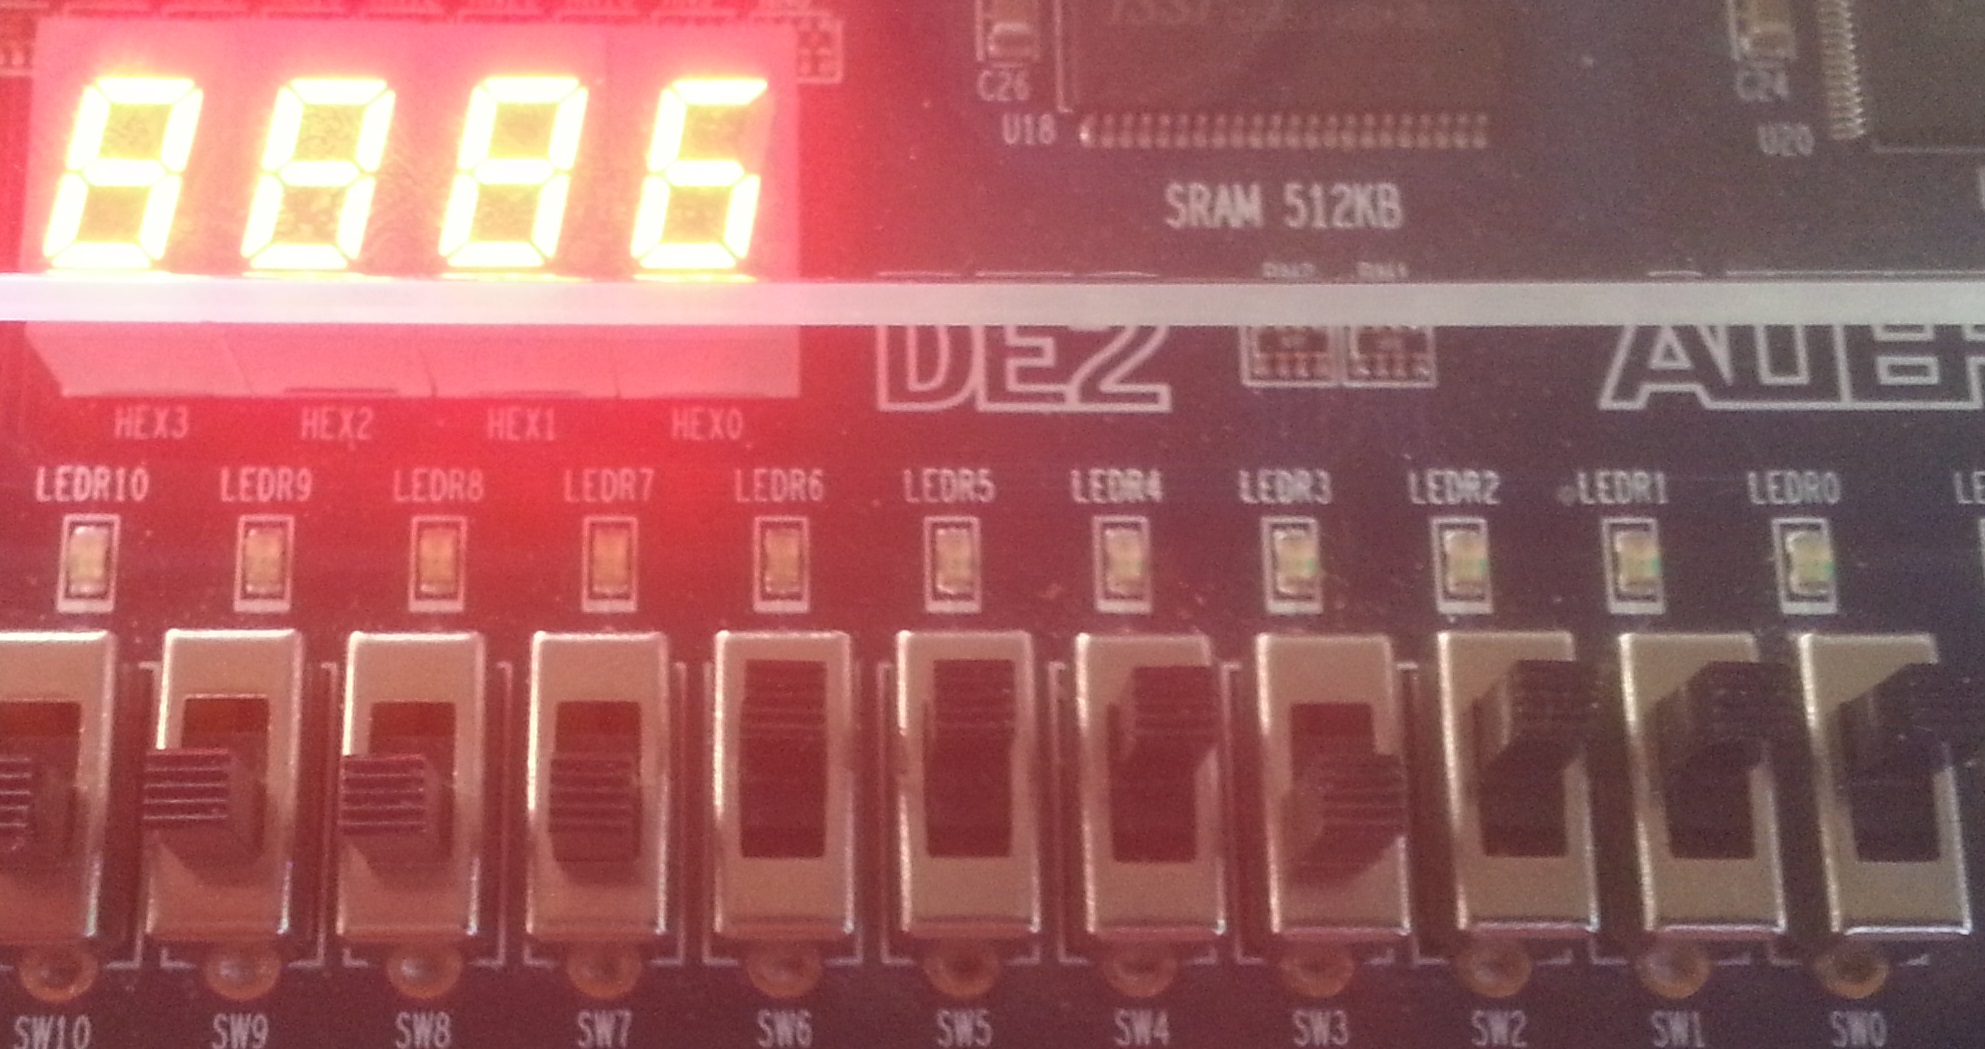
\includegraphics[scale=0.2]{pictures/Oevelse5/opg5/1count_6.JPG}
		\caption{}
		\label{fig:1count6}
	\end{figure}
	\begin{figure}[h]
		\centering
		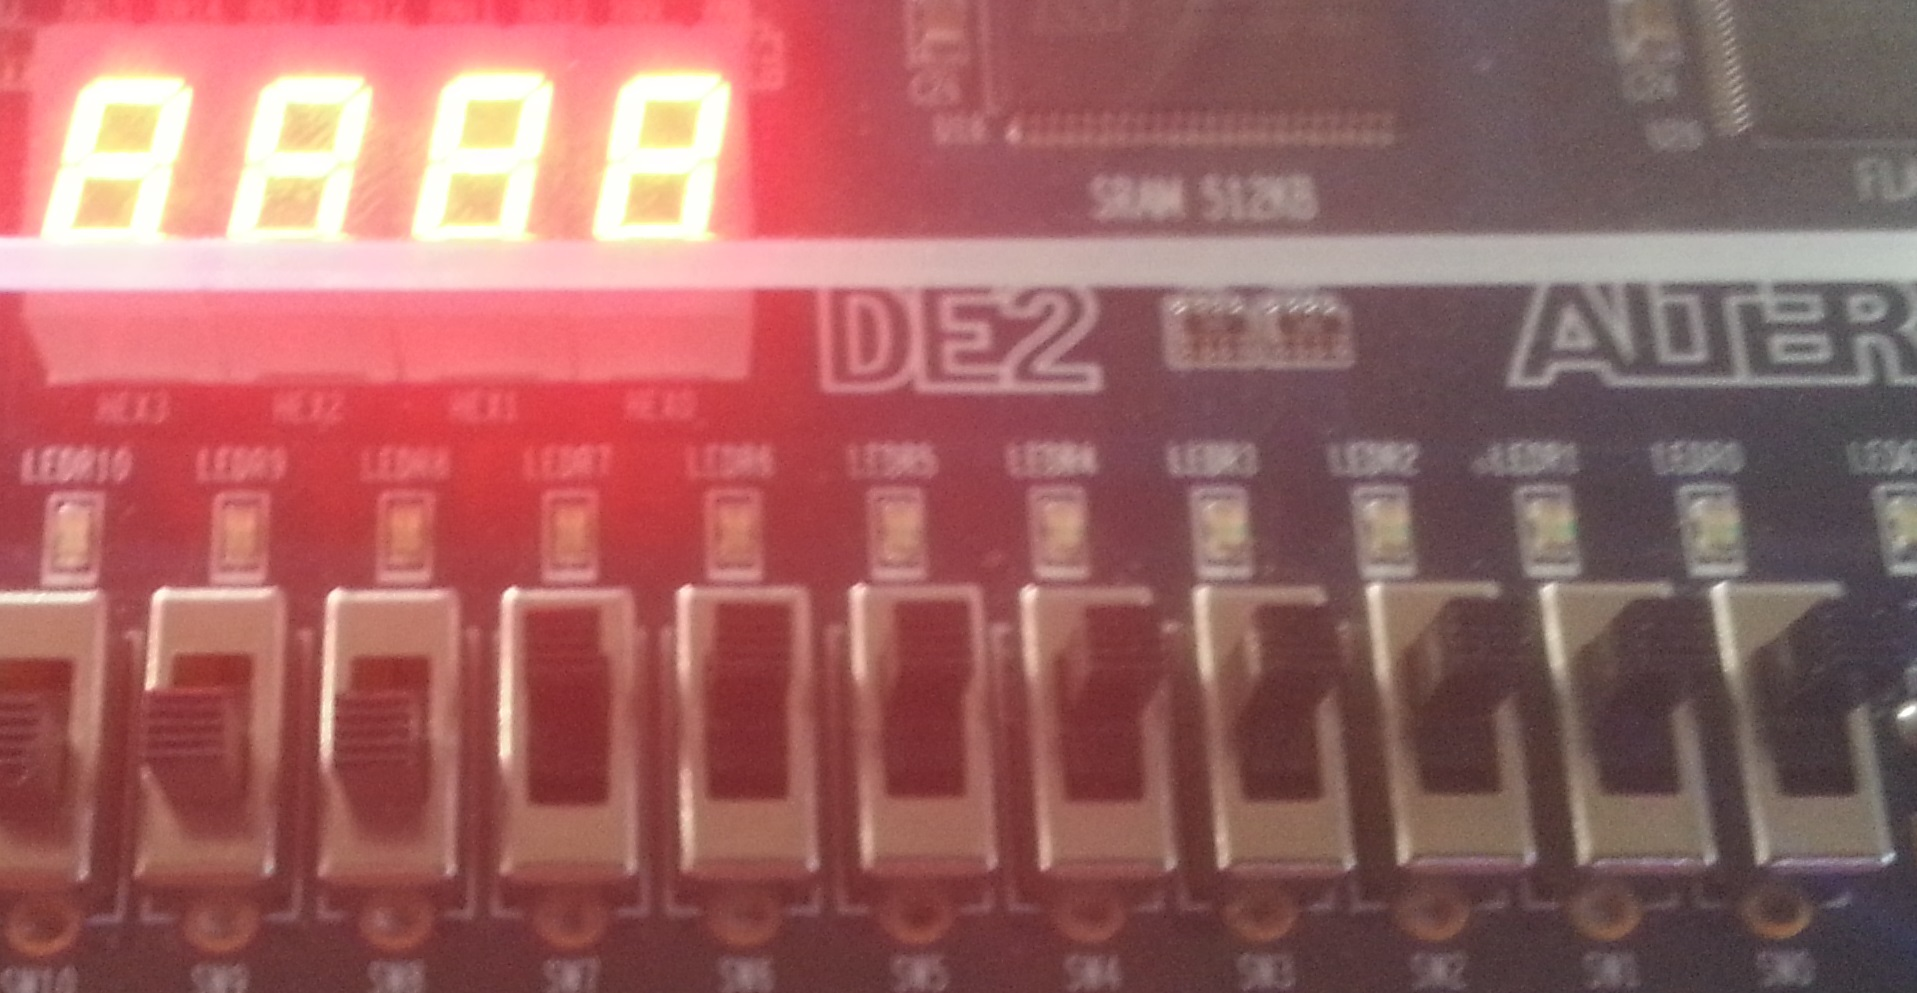
\includegraphics[scale=0.2]{pictures/Oevelse5/opg5/1count_8.JPG}
		\caption{}
		\label{fig:1count8}
	\end{figure}
	\begin{figure}[h]
		\centering
		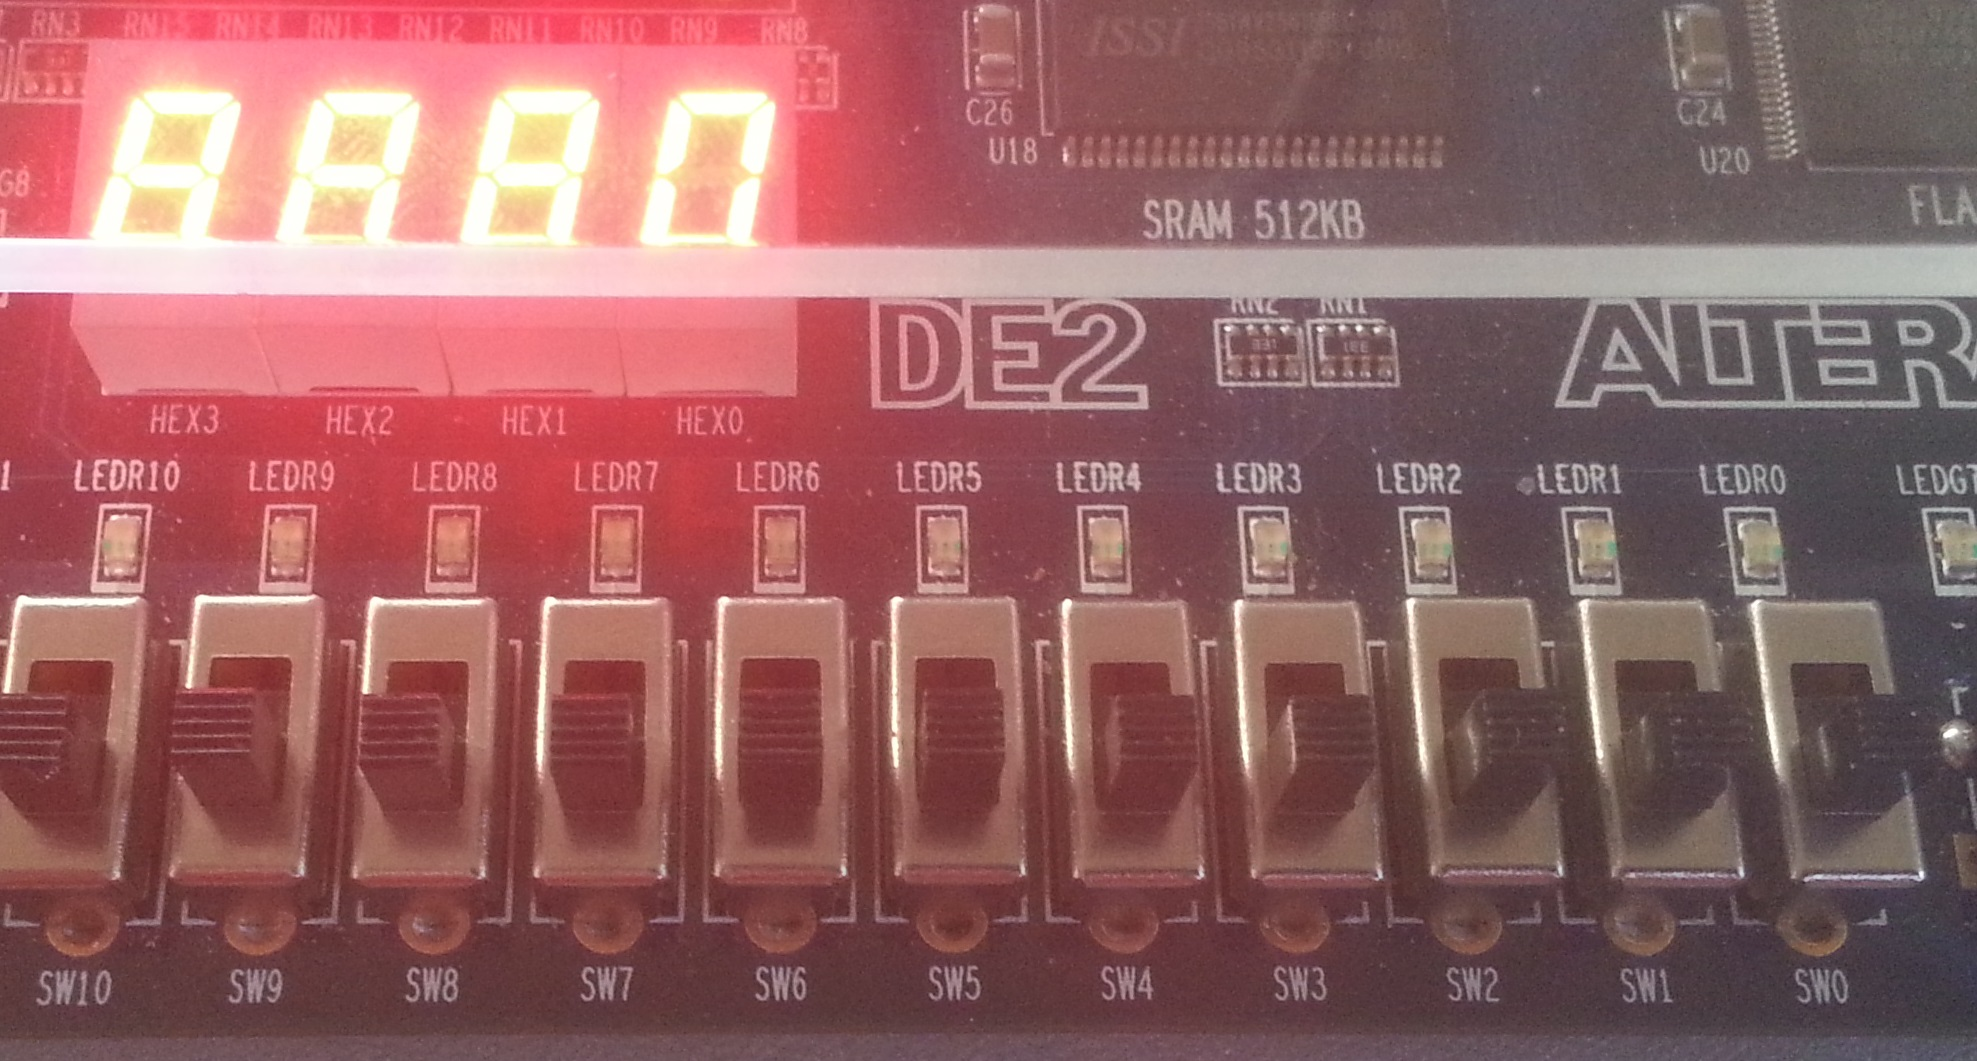
\includegraphics[scale=0.2]{pictures/Oevelse5/opg5/1count_0.JPG}
		\caption{}
		\label{fig:1count0}
	\end{figure}
\end{enumerate}